\documentclass{article}

\usepackage{graphicx}
\usepackage{indentfirst}
\usepackage[a4paper, total={6in, 8in}]{geometry}
\usepackage{hyperref}
\usepackage{fancyhdr}
\usepackage{xepersian}
\settextfont{XB Zar.ttf}
\setlatintextfont{Times New Roman.ttf}

\begin{document}


%title page%
\begin{titlepage}
	\begin{center}
		\vspace{0.2cm}
		
		
\includegraphics[width=0.4\textwidth]{sharif.png}\\
		\vspace{0.2cm}
		\textbf{ \Huge{آزمایش شماره 3}}\\
		\vspace{0.25cm}
		\textbf{ \Large{آز شبکه - دکتر بردیا صفایی}}
		\vspace{0.2cm}
		
		
		\large \textbf{دانشکده مهندسی کامپیوتر}\\\vspace{0.1cm}
		\large   دانشگاه صنعتی شریف\\\vspace{0.2cm}
		\large   ﻧﯿﻢ‌سال اول ۰۱-۰۲ \\\vspace{0.10cm}
		\large{\href{mailto:mehrshad.mirmohammadi@gmail.com}{مهرشاد میرمحمدی - 98109634}}\\
		\large{\href{mailto:parhaamsaremi@gmail.com}{پرهام صارمی - 97101959}}\\
		\large{\href{mailto:mofayezi.m@gmail.com}{محمدرضا مفیضی - 98106059}}\\
	\end{center}
\end{titlepage}
%title page%

\newpage

%pages header
\pagestyle{fancy}
\fancyhf{}
\fancyfoot{}
\setlength{\headheight}{59pt}
\cfoot{\thepage}
\lhead{آزمایش شماره 3}
\rhead{
\includegraphics[width=0.1\textwidth]{sharif.png}\\
		دانشکده مهندسی کامپیوتر
}
\chead{آز شبکه}
%pages header
\section{wireshark}
\subsection{بدست‌آوردن captcha}

همانند دستور عمل می‌کنیم، با این تفاوت که به جای استفاده ازهمانند دستور عمل می‌کنیم، با این تفاوت که به جای استفاده از SSL ، از TLS استفاده می‌کنیم. دلیل آن هم این است که SSL منسوخ شده و TLS جای آن را گرفته است. همچنین این پروتکل در ورژن wireshark مورد استفاده موجود نبود. لیست فایل‌‌های استخراج شده و captchaی بدست‌آمده را می‌توان در تصاویر \ref{fig:1} و \ref{fig:captcha} دید.

\begin{figure}[h!]
	\centering
	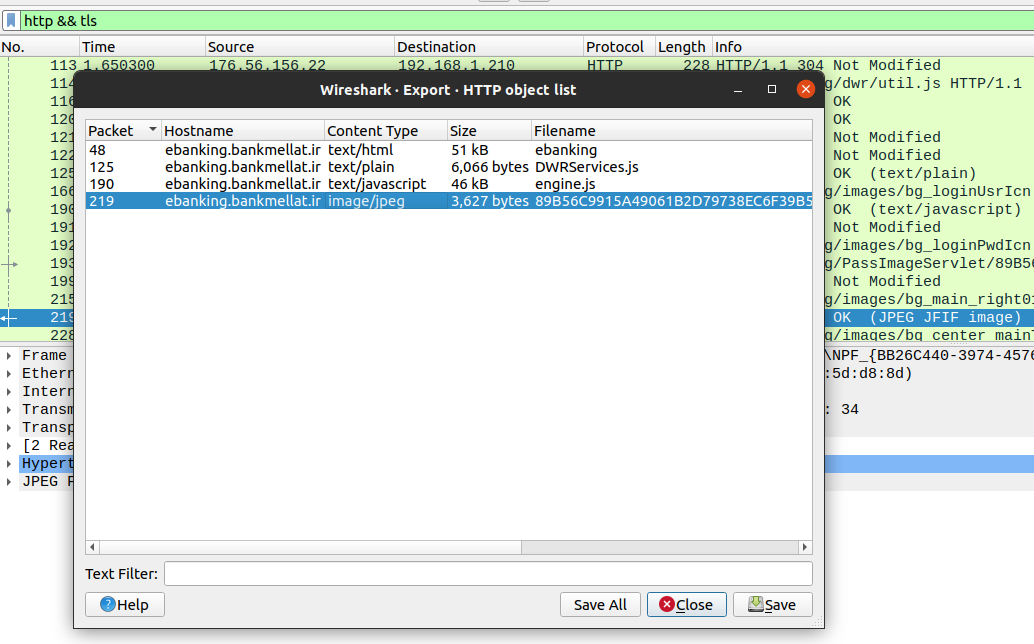
\includegraphics[width=0.9\textwidth]{src/1.png}
	\caption{پنجره‌ی ذخیره‌سازی فایل‌های بدست‌آمده.}
	\label{fig:1}
\end{figure}
\begin{figure}[h!]
	\centering
	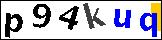
\includegraphics[width=0.5\textwidth]{src/captcha.jpeg}
	\caption{عکس بدست‌آمده.}
	\label{fig:captcha}
\end{figure}

\subsection{سوال‌ها}
\begin{enumerate}
    \item {
    این اطلاعات و آماره‌‌ها را می‌توان از طریق منو‌ی statistics موجود در wireshark بدست آورد. برای مثال با استفاده از بخش سلسله مراتب پروتکل‌ها می‌توان دید پروتکل‌های استفاده شده کدام‌‌ها هستند، از هر کدام چند پکت موجود است و چند درصد از پکت‌ها و بایت‌ها برای آن بوده است. تصویر \ref{fig:2} نمونه خروجی این ابزار است. همچنین با استفاده از باقی ابزار‌‌ها می‌توان اطلاعات دیگری همانند طول بسته‌ها، ترافیک و تعداد بسته‌های بین بخش‌های مختلف شبکه، زمان بین پاسخ‌ها و … بدست‌آورد.
    \begin{figure}[h!]
    	\centering
    	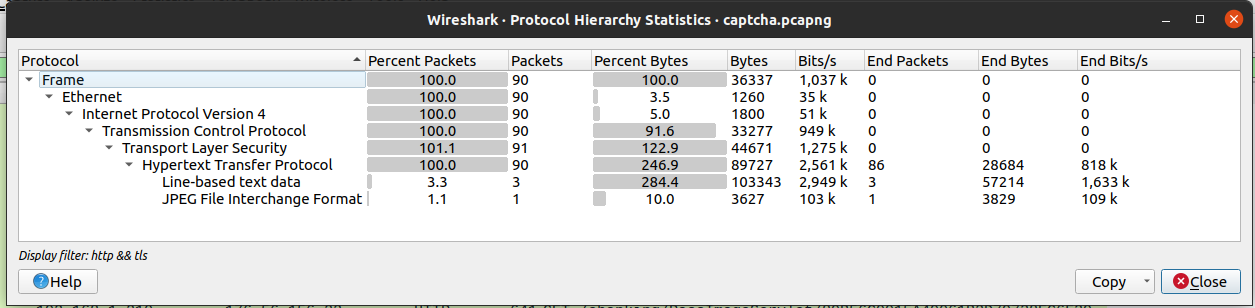
\includegraphics[width=0.9\textwidth]{src/2.png}
    	\caption{statistics > Protocols Hierarchy}
    	\label{fig:2}
    \end{figure}
    }
    \item {
    پروتکل RTP یک پروتکل بیدرنگ برای انتقال صدا و تصویر در شبکه‌ها با بستر IP است. این پروتکل معمولا بر پایه‌ی UDP است و برای streaming استفاده می‌شود. همچنین معمولا برای کنترل ترتیب رسیدن بسته‌ها، از پرتوکل RTCP هم به همراه آن استفاده می‌شود.
    
    در wireshark می‌توان با رفتن به Teⅼephony سپس RTP و سپس RTP streams اطالعات مربوط به آن را یافت. اطلاعاتی مانند آدرس و پورت مبدا و مقصد، میانگین و حداکثر jitter ، گمشدگی و …‬ که در تصویر \ref{fig:3} هم می‌توان دید. همچنین امکان ضبط و بخش محتوا به صورت مستقیم هم موجود است.
    \begin{figure}[h!]
    	\centering
    	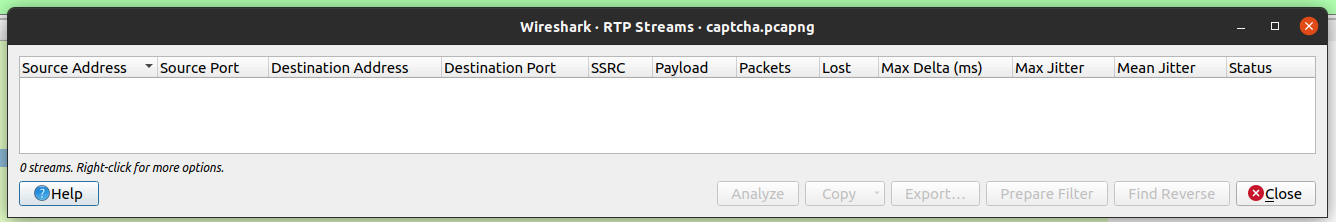
\includegraphics[width=0.9\textwidth]{src/3.png}
    	\caption{‫‪Telephony‬‬ ‫>‬ ‫‪RTP‬‬ ‫>‬ ‫‪RTP‬‬ ‫‪Streams}
    	\label{fig:3}
    \end{figure}
    }
\end{enumerate}

\end{document}
